% Background

\chapter{Background} % Main chapter title

\label{Chapter2} % For referencing the chapter elsewhere, use \ref{Chapter2} 

\lhead{Chapter 2. \emph{Background}} % This is for the header on each page - perhaps a shortened title

%----------------------------------------------------------------------------------------

In this section, we go investigate different types of music games, along with a deeper look into Guitar Hero, on which we base our main concept for the gameplay. This is followed by a discussion of the most applicable publications in music analysis, on finding the main melody in a musical track in particular.


\section{Music Video Games }

A music video game can be defined as a type of game that uses music or rhythm as an integral part of gameplay. This may involve pressing buttons in time with a song, whether on a conventional controller, and instrument controller or some kind of dance mat, singing into a microphone or creating original music. Players can often perform different parts of the same song together in local multiplayer games or over the Internet, providing enjoyable social experiences. [2]

Some games exhibit a sandbox style that encourages a free-form gameplay approach whereas other a hybrid style, which combines musical elements with more traditional genres, for example puzzle games or shooters. 

Below we will briefly go over different types of music video games that can be found on the market.


\subsection{Music Memory Games}

The goal of the music memory game is to score player on their musical memory. Music track is presented to the user who then has to provide an appropriate response to each prompt from the game. Games may be based on different primary musical aspect (whether it is the rhythm, pitch or volume). However, a vast majority of the releases available on the market are rhythm-based.

\begin{wrapfigure}{r}{0.45\textwidth}
  \vspace{-10pt}

  \begin{center}
    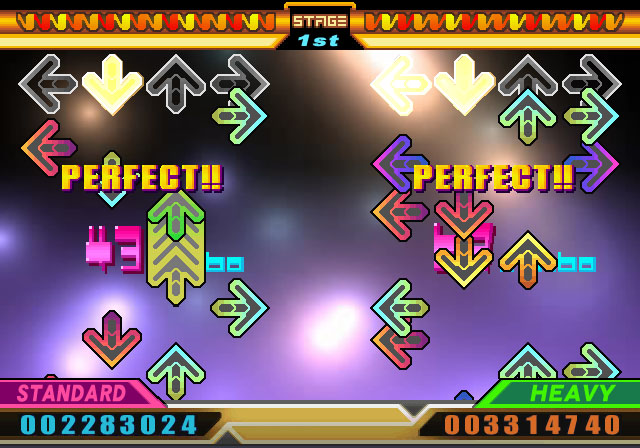
\includegraphics[width=0.43\textwidth]{Figures/dancedancerevolution}
  \end{center}
  \caption{Screenshot from Dance Dance Revolution, an example of a rhythm music game. [11]}
\end{wrapfigure}

Rhythm games typically focus on dance or the simulated performance of musical instruments, and require players to press buttons in a sequence dictated on the screen. Doing so causes the game's protagonist or avatar to dance or to play their instrument correctly, which increases the player's score. [10] An example of such games could be Guitar Hero or Dance Dance Revolution.


\subsection{Free Form Music Games}

In free form music games, the main task of the user is to create content. This form of music game is often compared to non-game music synthesisers. Free form music games are somewhere between generative hybrid music games and non-game utilities, depending on the degree to which their gameplay relies on a driving underlying plot-line.


\subsection{Hybrid Music Games}

Hybrid music games are characterised by substantial and meaningful interactions between a player and the music game in a game that apparently belongs to a non-musical genre. This type of games can be further split into two sub-types.


Generative music video games make use of user’s actions. By monitoring interaction with the surroundings in the game, the mechanism generates sounds that are then integrated into the soundtrack, permitting the player’s direct interaction with the score. This encourages the creation of a synesthetic experience — when upon stimulation of one sense others activate, causing an involuntary experience. An example of such game could be Rez, which is a simple rail shooter. However, thanks to integrating sounds generated by player completing the normal task of rail-shooting, the score is dynamic.

Reactive music games, in contrast to generative one, employ music to determine the gameplay. In such games, the player takes cues from soundtrack to devise his gameplay. For example, iS - internal section, uses the music to determine the dynamic of the non-musical components of the game.

\begin{figure}
        \centering
        \begin{subfigure}[b]{0.48\textwidth}
                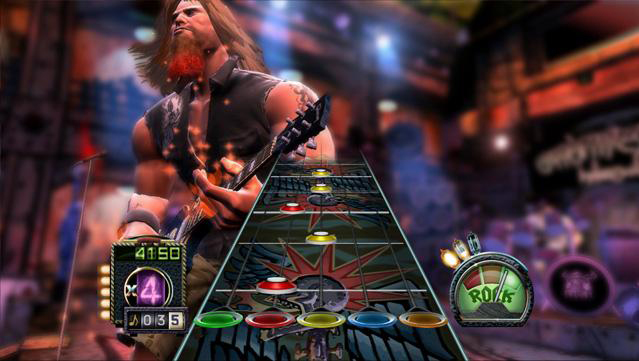
\includegraphics[width=\textwidth]{Figures/guitarhero}
                \caption{Screenshot from Guitar Hero - player is attempting to play a song. [8]}
                \label{fig:Guitar Hero screenshot}
        \end{subfigure}%
        ~ %add desired spacing between images, e. g. ~, \quad, \qquad, \hfill etc.
          %(or a blank line to force the subfigure onto a new line)
        \begin{subfigure}[b]{0.48\textwidth}
                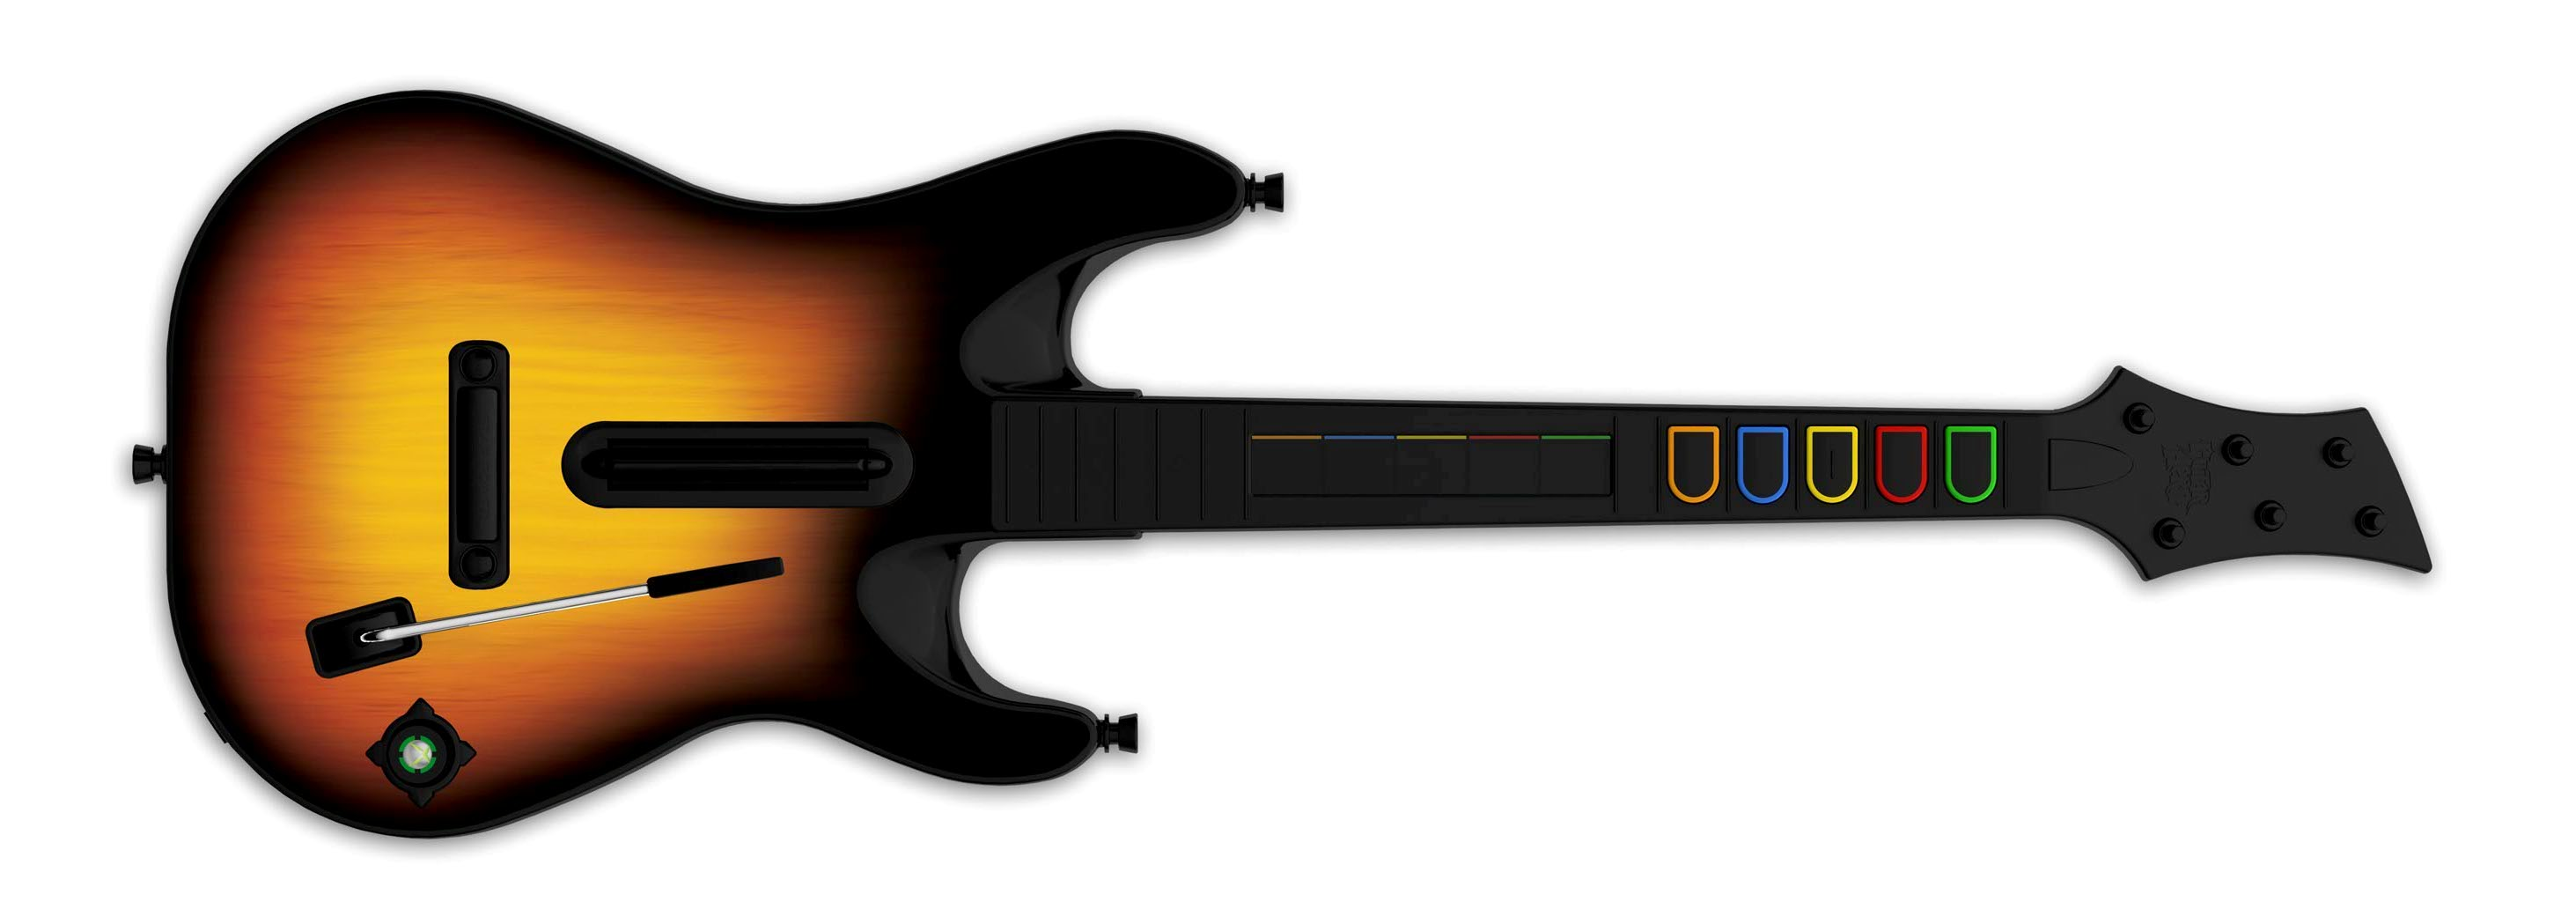
\includegraphics[width=\textwidth]{Figures/controller}
                \caption{A guitar shaped controller used in the game. [7]}
                \label{fig:Controller}
        \end{subfigure}
          \caption{Guitar Hero components}
        ~ %add desired spacing between images, e. g. ~, \quad, \qquad, \hfill etc.
\end{figure}

  \vspace{40pt}

\section{Case Study - Guitar Hero}

Guitar Hero is one of the most popular franchises in the history of music games. The first of the series was published in 2005 by RedOctane and Harmonix. In the games, players instrument-shaped game controllers to simulate playing the instruments across numerous rock music songs. It is widely considered a highly entertaining game fully embracing the rhythm-based music game.


\subsection{The Controller}


Rather than a typical gamepad, Guitar Hero uses an instrument-shaped controller (guitar in the earlier releases, bass, microphone and drums in more recent ones). Playing the game with the guitar controller simulates playing an actual guitar, except it uses five coloured "fret buttons" and a "strum bar" instead of frets and strings, and an analogous mapping for the other instruments. They incorporate most of the real life techniques and motions that an instrumentalist would perform on a real instrument.


\subsection{The Gameplay}

The actual game itself works exactly as many other music titles do. At the bottom of the screen, a number of (varying depending of level of difficulty) buttons is shown. In each attempt, a series of notes moves across the screen and when a note aligns with a button, player is supposed to press a corresponding button, gaining points depending on the accuracy. If the player failed to achieve a certain amount of notes — his performance meter stays low for a longer time, he loses the game.

However, there are a couple minor improvements that Harmonix has made to the general music game formula. By acing certain notes in a song, a player is able to build up Star Power, which when unleashed, doubles up current point multiplier. Star Power also adds a bit of a strategic element —player not only earns more points when it is activated, but he can also raise your performance meter faster, enabling him to last longer when encountering a trickier part of a song.


\subsection{The Critique}

Without a doubt, Guitar Hero features a great selection of music. However, there will always be tracks missing, regardless of how many versions of Guitar Hero are released. People have different tastes and limiting a game to a set of tracks that everybody is supposed to enjoy is a really hard task. 

Some more advanced users familiar with Computer Science attempted to transcribe songs and to create new levels. However, this process is really difficult, especially for non computer scientists, discouraging an average user from fully making use of game’s capabilities. The producers, seeing the tendency, started releasing the in-app purchases to enable the players to extend their library and thus, keep the users. 

Implementing a feature of uploading some music preferred by the player would definitely improve user satisfaction. However, this might have not been achieved yet as the task itself is quite complex. Moreover, enabling the users to load in some music would deprive the company of their income sources.


\section{Introduction to Melody Extraction}

For a long time people were researching ways of estimating the fundamental frequency, be it with monophonic music recording or multi-pitch estimation. Melody extraction differs from both of those problems — unlike monophonic pitch estimation it handles polyphonic tracks and in contrast to multi-pitch estimation, it must also include a mechanism for source identification, to spot the voice carrying the melody within the polyphony.
To be able to evaluate the performance of the new algorithms, annual Music Information Retrieval Evaluation eXchange (MIREX) has been running since 2005. In this campaign, different models are evaluated against the same sets of music collections in order to obtain a quantitative comparison between methods and assess the accuracy of the current state-of-the-art in melody extraction. [14]


\subsection{Melody}

The concept of “melody” ultimately relies on the judgement of people listening. This is why it will vary depending on the application context - whether we want to determine symbolic melodic similarity or transcribe a music track. 

In order to have a clear framework to work within, the Music Information Retrieval (MIR) community has adopted in recent years the definition proposed by [4], “...the melody is the single (monophonic) pitch sequence that a listener might reproduce if asked to whistle or hum a piece of polyphonic music, and that a listener would recognise as being the ‘essence’ of that music when heard in comparison”.

In practice, research has focused on “single source predominant fundamental frequency estimation” — which means a search for a main melody coming from a single sound source throughout the song analysed. As we can see, the subjective element is still present in this description of a melody as there might not be a definite way of deciding what predominant is. However, it fits well with our project’s objective — generating a game level based on changes in the pitch.


\subsection{Polyphonic Music}

Polyphony is a word derived from Greek poluph\={o}nosis meaning more than one sound — a texture consisting of two or more simultaneous lines of independent melody. This can be contrasted with homophony, where musical parts move generally in the same rhythm and one dominant melodic voice is accompanied by chords or monophony, where only one voice is found. 

However, in our case, the term polyphonic will simply refer to any type of music in which two or more notes can be played simultaneously. This can be achieved either by playing in different instruments (for example, voice, guitar and bass) or a single instrument capable of playing more than one more at a time (like a piano).


\subsection{Pitch, Tones, Fundamental Frequency}

Pitch is the most natural way of ordering sounds on a frequency-related scale. If sounds whose frequency is clear and stable enough to be distinguished from noise, they can be compared among  one another as “lower” or “higher”. Pitch is not an objective physical property — it depends on anatomy and physiology of the auditory system, which is a subject of an extensive study called psychoacoustics. 

A semitone is the smallest musical interval commonly used in Western tonal music. Two semitones constitute a tone.

The fundamental frequency $f_{\text{0}}$ is defined as the lowest frequency of a periodic waveform. A harmonic (or a harmonic partial) is any of a set of partials that are whole number multiples of a common fundamental frequency. This set includes $f_{0}$, which is a whole number multiple of itself (1 times itself).

Fundamental frequency can be thought of as the physical property most closely related to perception of pitch. This is why in this context pitch and fundamental frequency can be used interchangeably.


\subsection{Filter}

Any medium through which the music signal passes, whatever its form, can be regarded as a filter. However, we do not usually think of something as a filter unless it can modify the sound in some way. 

A digital filter is a filter that operates on digital signals, such as sound represented inside a computer. It is a computation which takes one sequence of numbers (the input signal) and produces a new sequence of numbers (the filtered output signal). [15]


\subsection{Short Time Fourier Transform}

Short-time Fourier transform (STFT), is a signal processing method which is used in analysis of non-stationary signals with statistic characteristics varying with time.
In particular, STFT extracts several frames of the signal to be analysed with a window that moves with time. If we set the window size to be narrow enough, each frame extracted can be viewed as stationary so that Fourier transform can be used. With the window moving along the time axis, the relation between the variance of frequency and time can be identified. [6]

The short time Fourier transform of a time-domain signal $y$ is denoted by the matrix $F \times N$, $F$ being the Fourier transform size and $N$ the number of analysis frames.

\section{Main Melody Extraction from Polyphonic Music}
\subsection{Source Separation Based Approach}

\begin{wrapfigure}{r}{0.5\textwidth}
  \vspace{-50pt}

  \begin{center}
    \includegraphics[width=0.48\textwidth]{Figures/durrieudiagram}
  \end{center}
  \caption{Outline of system proposed by Durrieu: X is the STFT of the mixture sygnal, $p(\Xi|X)$ the posterior probability of a given melody sequence, and $\hat{\Xi} $ the desired smooth melody sequence.}
\end{wrapfigure}


In polyphonic tracks the main melody can be represented by a specific source/filter model. In case of the leading vocal part, the vocal cords are treated as a source and the voice tract as a linear acoustic filter.

In their paper from 2011 [5], authors presented an algorithm in which they assume that at any given time the signal observed is a mixture of two elementary signals - one corresponding to the main source and one to the background music. Therefore, the signal can be represented in an equation $x(t) = v(t) + m(t)$, where $v(t)$ stands for the source of the main melody and $m(t)$ is the background music. Interestingly, this equation also holds for the short time Fourier transform (STFT)  $X$, $V$ and $M$ respectively: $X = V + M$. The models proposed by Durrieu essentially aim at constraining the shapes of these STFT using temporal and spectral constraints. 


The likelihood of the vocal part V is calculated using two different frameworks. 

The first submission uses the source/filter Gaussian scaled mixture model (GSMM). In this model the source element refers to the excitation of the vocal folds and is therefore linked to the fundamental frequency of the sound $f_{\text{0}}$, while the filter part is characteristic of the vocal tract shape. This space of possibilities is then discretised so that we consider one possible filter frequency response, which is then used to calculate the likelihood of the vocal part knowing the filter and $f_{\text{0}}$.

Fig 2.4. A) shows the diagram of the GSMM model for the main voice part. Each source excitation $u$ is filtered by each filter $k$. The amplitudes for a frame $n$ and for all the couples $(k, u)$ are then applied to each of the output signals. At last a “state selector” sets the active state for the given frame.

The second model was derived from the first one to find a solution that would be more efficient to compute. The authors came up with a formulation that keep the source/filter model within an instantaneous mixture framework (IMM). In this model, for each source a set of filters is defined and at each frame, once every source is filtered and multiplied by a given amplitude, they are all added together.

The background music signal $m(t)$ can be thought of as a mixture of $R$ independent Gaussian sources $m_{r}(t)$. 
Each of the sources is centred and characterised by its power spectral density (PSD), which describes how the power of a signal or time series is distributed over the different frequencies. PSD can be estimated using a Covariance Method.
Due to the linearity of the Fourier transform, $M(f,t)$, the STFT of $m$, is also the instantaneous mixture of the $R$ spectra $M_{r}(f,t)$ of the sources: $M_{r}(f,t)$.
This together with STFT and an amplitude coefficient associated with each source is used to calculate the likelihood for each of the frequency bins. Let $M_{t}(f)$ be the STFT of the background signal at frame $t$ and frequency bin $f$, then we write its likelihood.

\begin{figure}
        \centering
        \begin{subfigure}[b]{0.47\textwidth}
                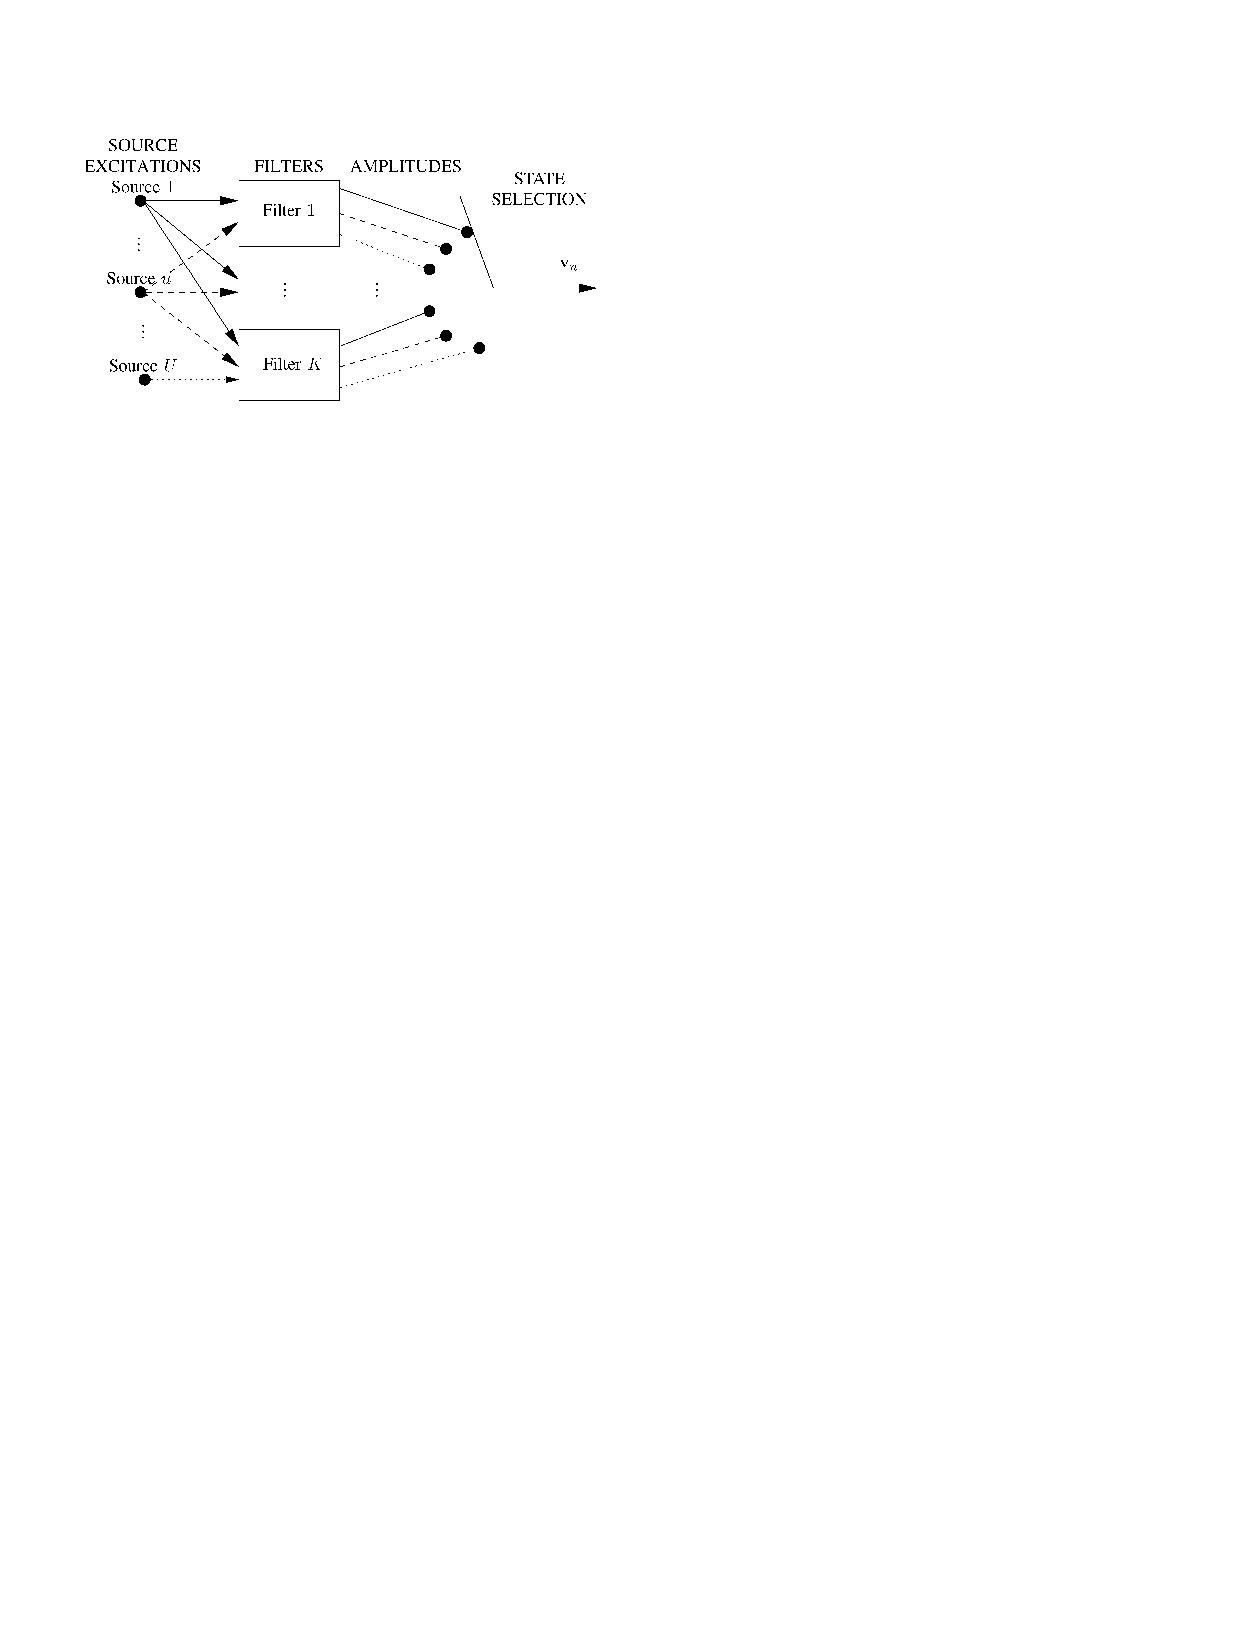
\includegraphics[width=\textwidth]{Figures/gsmm}
                \caption{Schematic principle of the generative GSMM. Each source u is filtered by each filter k. For frame n, the signal is then multiplied by a  given amplitude and a "state selector" then chooses the active state.}
                \label{fig:Guitar Hero screenshot}
        \end{subfigure}%
        ~ %add desired spacing between images, e. g. ~, \quad, \qquad, \hfill etc.
          %(or a blank line to force the subfigure onto a new line)
        \begin{subfigure}[b]{0.47\textwidth}
                \includegraphics[width=\textwidth]{Figures/imm}
                \caption{Schematic principle of the generative IMM. At each frame, all the U sources, each filtered by K filters, are multiplied by amplitudes and added together to produce the leading voice signal.}
                \label{fig:Controller}
        \end{subfigure}
          \caption{Diagram of both models presented in the paper.}
        ~ %add desired spacing between images, e. g. ~, \quad, \qquad, \hfill etc.
\end{figure}

Once the parameters are estimated using the maximum likelihood criterion for each of the model, the Viterbi smoothing of the melody line is applied, obtaining a trade-off between the smoothness of the melody and its global energy in the signal. The Viterbi algorithm is a dynamic programming algorithm for finding the most likely sequence of hidden states – called the Viterbi path – that results in a sequence of observed events. [12]
 
The authors then parametrise the transitions between the possible main melody without disabling jumps from one note to the other.Usign Wiener filtering - digital signal processing reducing the noise, using an statistical estimate of the signal using a desired data without such noise, a framework is implemented to separate the source. This way separated signals are obtained. Computing the energy for each frame of the separated main melody and thereafter thresholding allowed to discriminate between spurious notes and true positives.


\subsection{Salience Based Approaches}

\begin{wrapfigure}{r}{0.5\textwidth}
  \vspace{-60pt}

  \begin{center}
    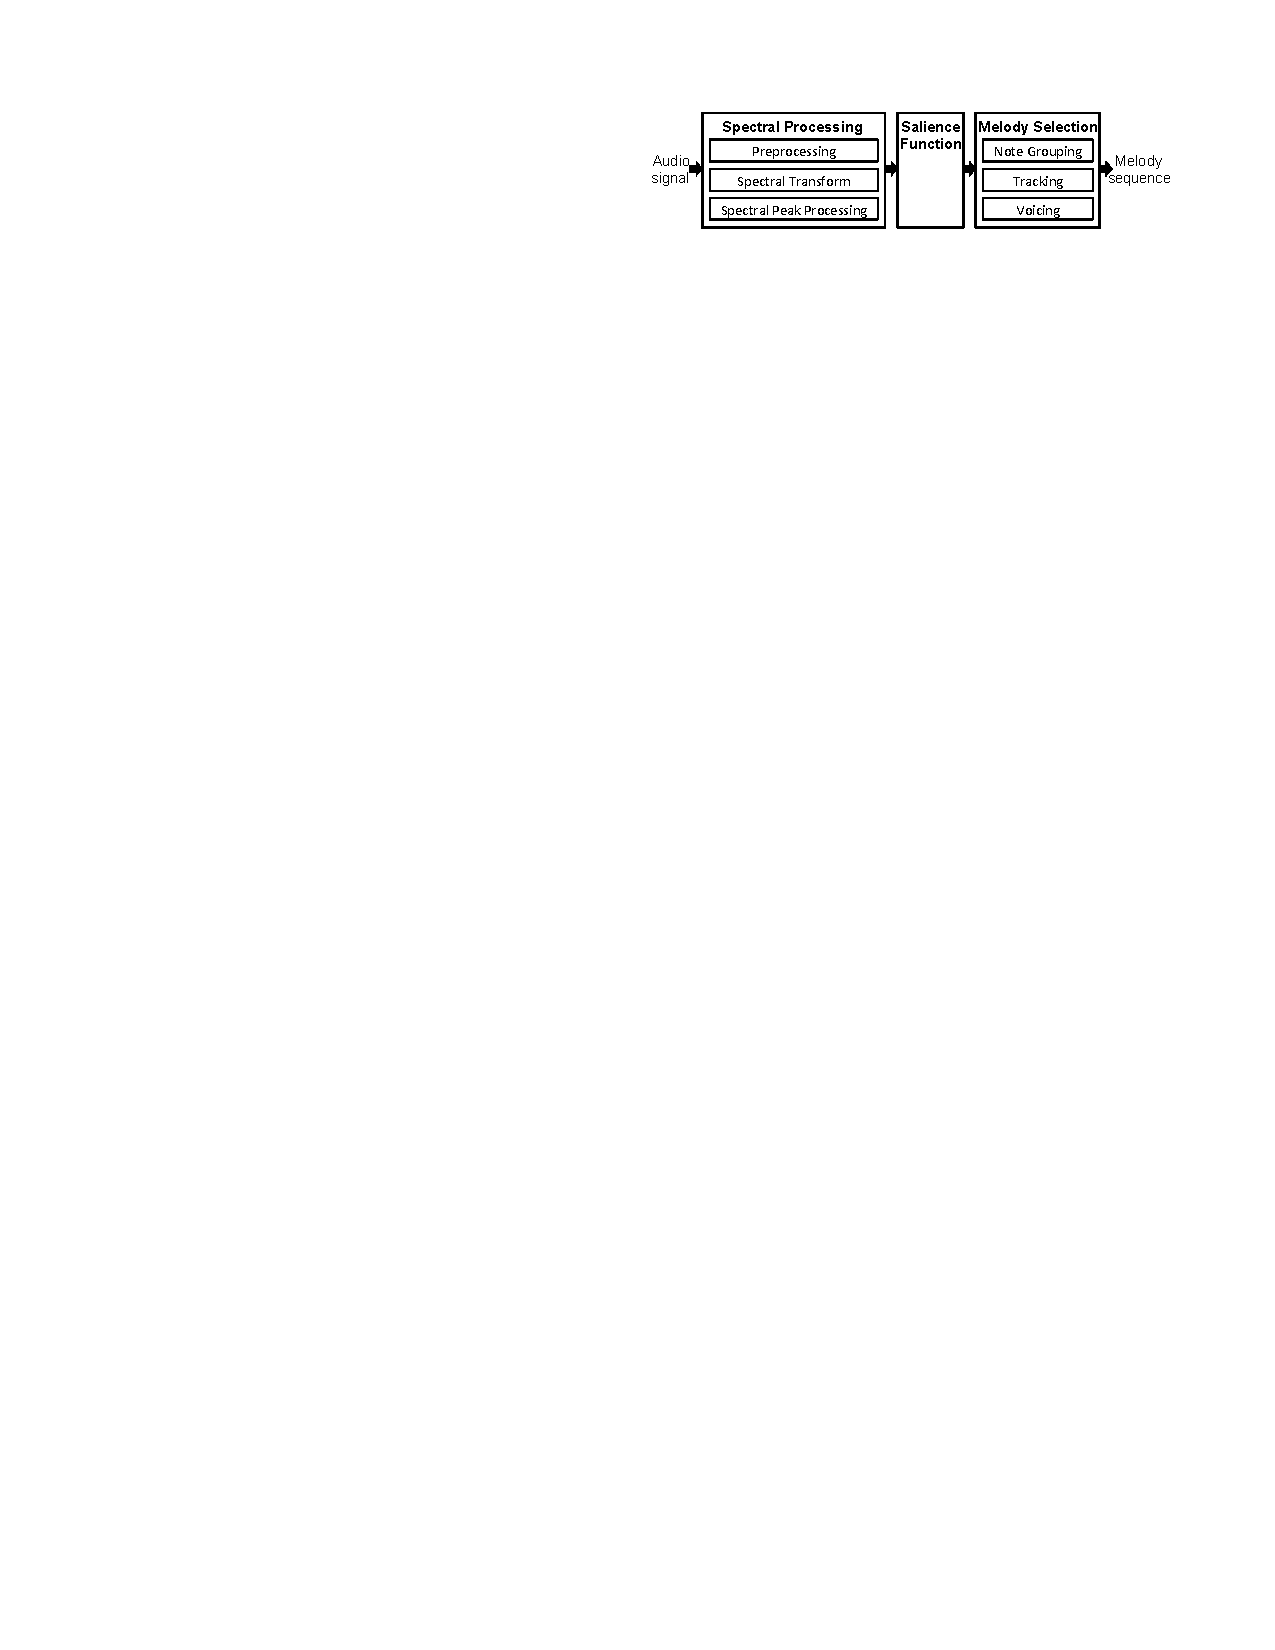
\includegraphics[width=0.48\textwidth]{Figures/salienceoveralldiagram}
  \end{center}
  \caption{Block diagram of four main blocks of the system by Salamon and G\'{o}mez: sinusoid extraction, salience function computation, pitch contour creaton and melody selection}
\end{wrapfigure}

This approach has been the most popular so far, with majority of algorithms evaluated at MIREX implementing it. It and can be split into several smaller stages, as seen in Figure 2.5. In particular, a method implemented in paper [9] seems to be quite promising.

Usually as a first step, some sort of preprocessing is applied to the audio signal, usually to enhance the frequency content where we expect to find the melody. In particular, Salamon and G\'{o}mez apply an equal loudness filter, which enhances the frequencies to which the human ear is more perceptually sensitive by taking a representative average of the equal loudness curves and filtering the signal by its inverse. 

This stage is followed by spectral transform — the signal is chopped into time frames and a transform function is applied to obtain a spectral representation of each frame.
This is achieved by applying the Short-Time Fourier Transform given by:

\begin{equation}
X_{l}(k) = \sum_{n=0}^{M-1} w(n) \times x(n + lH) e^{-j\frac{2 \pi}{N}kn}
\end{equation}

with a window length of 46.4ms. Here, $x(n)$ is the time signal, $w(n)$ the windowing function, $l$ the frame number, $M$ the window length, $N$ the FFT length and $H$ the hop size. Thanks to choosing a relatively small hop size we achieve sufficient frequency resolution to identify different notes while maintaining adequate time resolution to track pitch changes in the melody over a short time. 

Having done this, we move to frequency/amplitude correction, where the spectral peaks are detected and used to construct a salience function. To avoid a relatively large error in the estimation of the peak frequency caused by binning them in the process of FFT, peak’s instantaneous frequency and amplitude are calculated. 

Those three steps constitute the spectral processing. But at the core of the salience based algorithms lies the multi pitch representation, i.e. the salience function — a representation of pitch salience over time. The peaks of this function form the $f_{0}$ candidates for the main melody. In the algorithm described by Salamon and G\'{o}mez, this computation is based on harmonic summation, where the salience of  a given frequency is computed as a sum of the weighted energies found at harmonics (integer multiples) of that frequency. Using only the peaks for the summation allows us to discard less reliable values and apply further frequency corrections. 


\begin{wrapfigure}{l}{0.5\textwidth}
  \vspace{-20pt}

  \begin{center}
    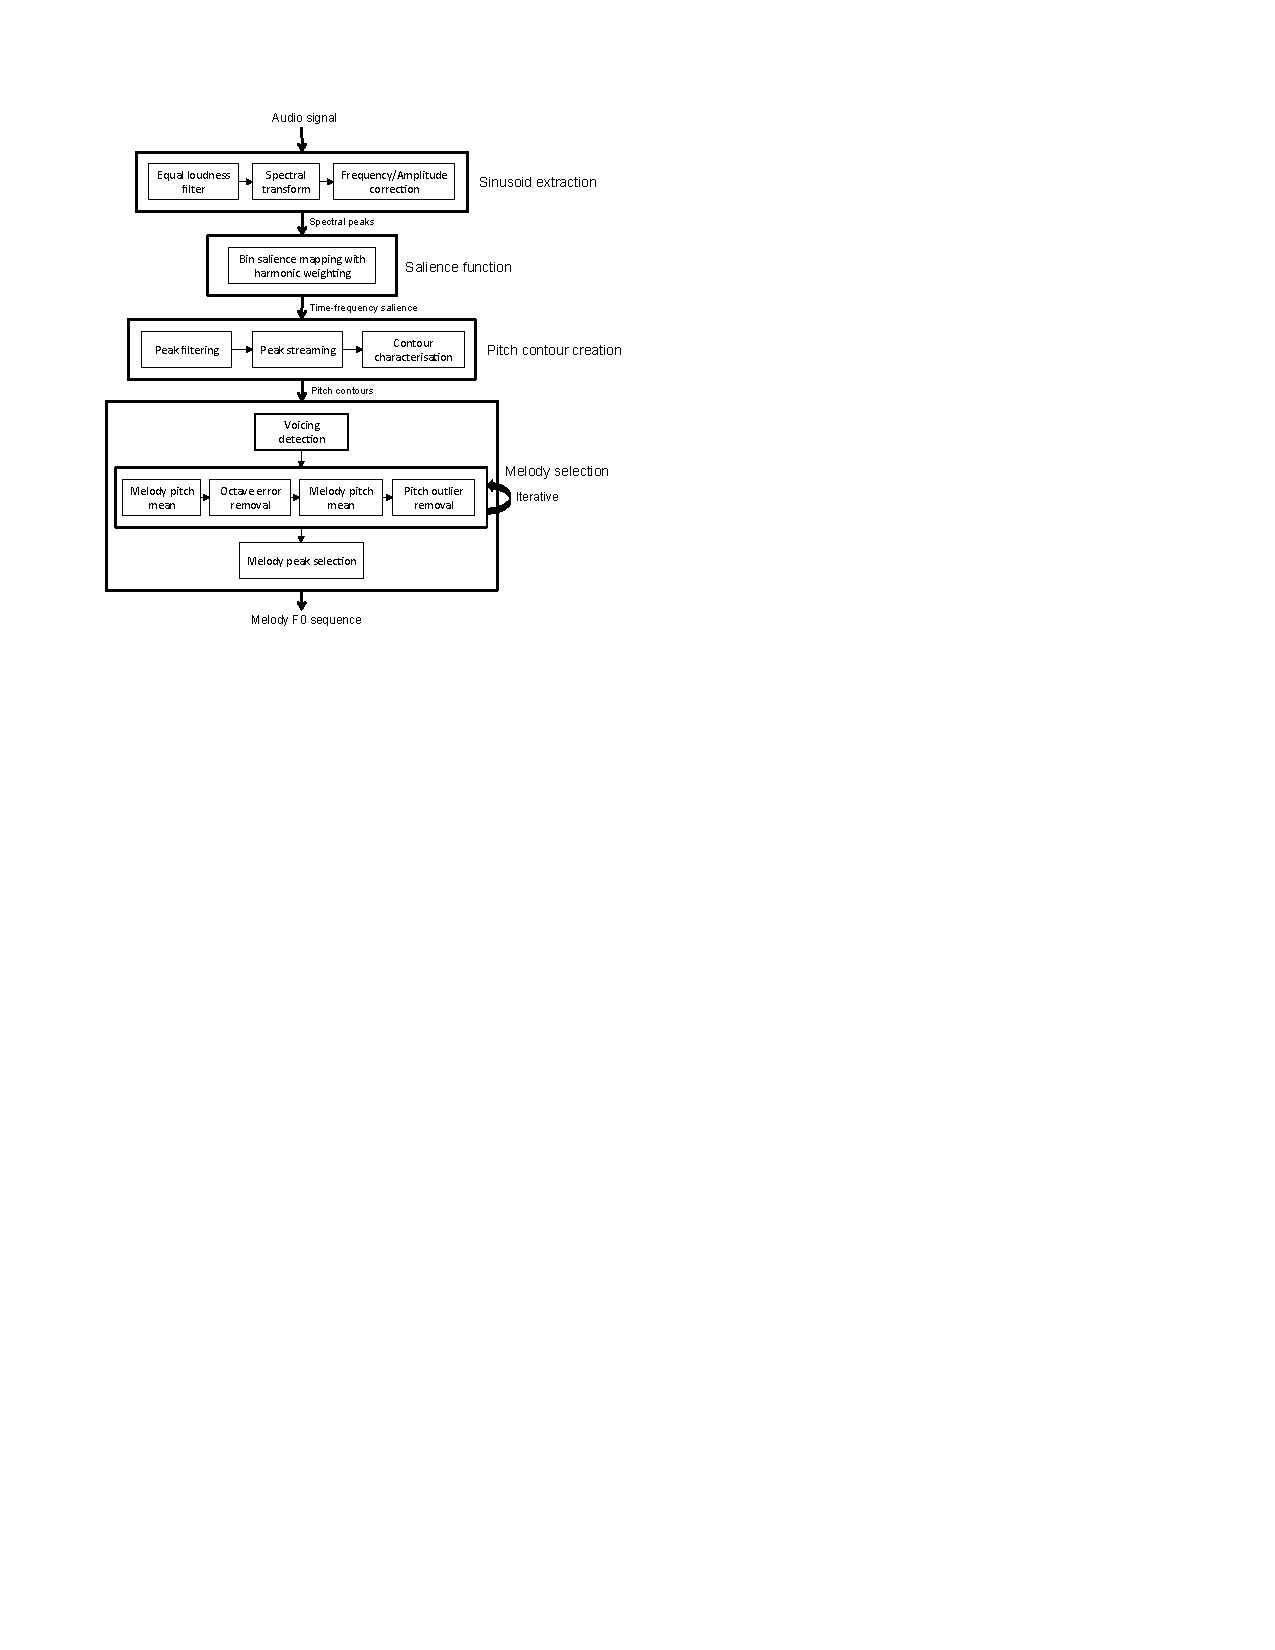
\includegraphics[width=0.48\textwidth]{Figures/salamon4blocksdiagram}
  \end{center}
  \caption{Block diagram of four main blocks of the system by Salamon and G\'{o}mez: sinusoid extraction, salience function computation, pitch contour creaton and melody selection}
\end{wrapfigure}

The salience function presented in the paper covers a pitch range of nearly five octaves from 55Hz to 1.76kHz.

Peaks of the salience function at each frame are now potential $f_{0}$ of the main melody. At this point some methods for melody extraction attempt to track the melody. However, Salamon and G\'{o}mez filter out the non-salient peaks, first by comparing them to the highest peak in the frame and then to a value computed using salience mean and standard deviation of all remaining peaks (in all frames). Now the peaks are grouped into pitch contours - time and pitch continuous sequences of salience peaks as shown in fFgure 2.7.

Having created the pitch contours, we are faced with the task of determining which one belongs to the main melody. The authors define features based on contour pitch, length and salience.

Given the peaks of the salience function, we now have to determine which pitch values belong to the melody. This process is initiated by grouping peaks into continuous pitch contours, out of which a melody is selected later. 

The consideration of various contour characteristics means accompanying instruments will not necessarily be selected as melody if they exhibit a certain melodic characteristic. For example, a contour produced by an accompanying violin with vibrato may still be discarded due to its pitch height. 

The next main block in this algorithm is the melody selection which is comprised of three steps: voicing detection, octave error minimisation/pitch outlier removal, and final melody selection.
As the name suggests, the aim of the voicing detection is to determine when the melody is present.

\begin{figure}[h!]
  \centering
    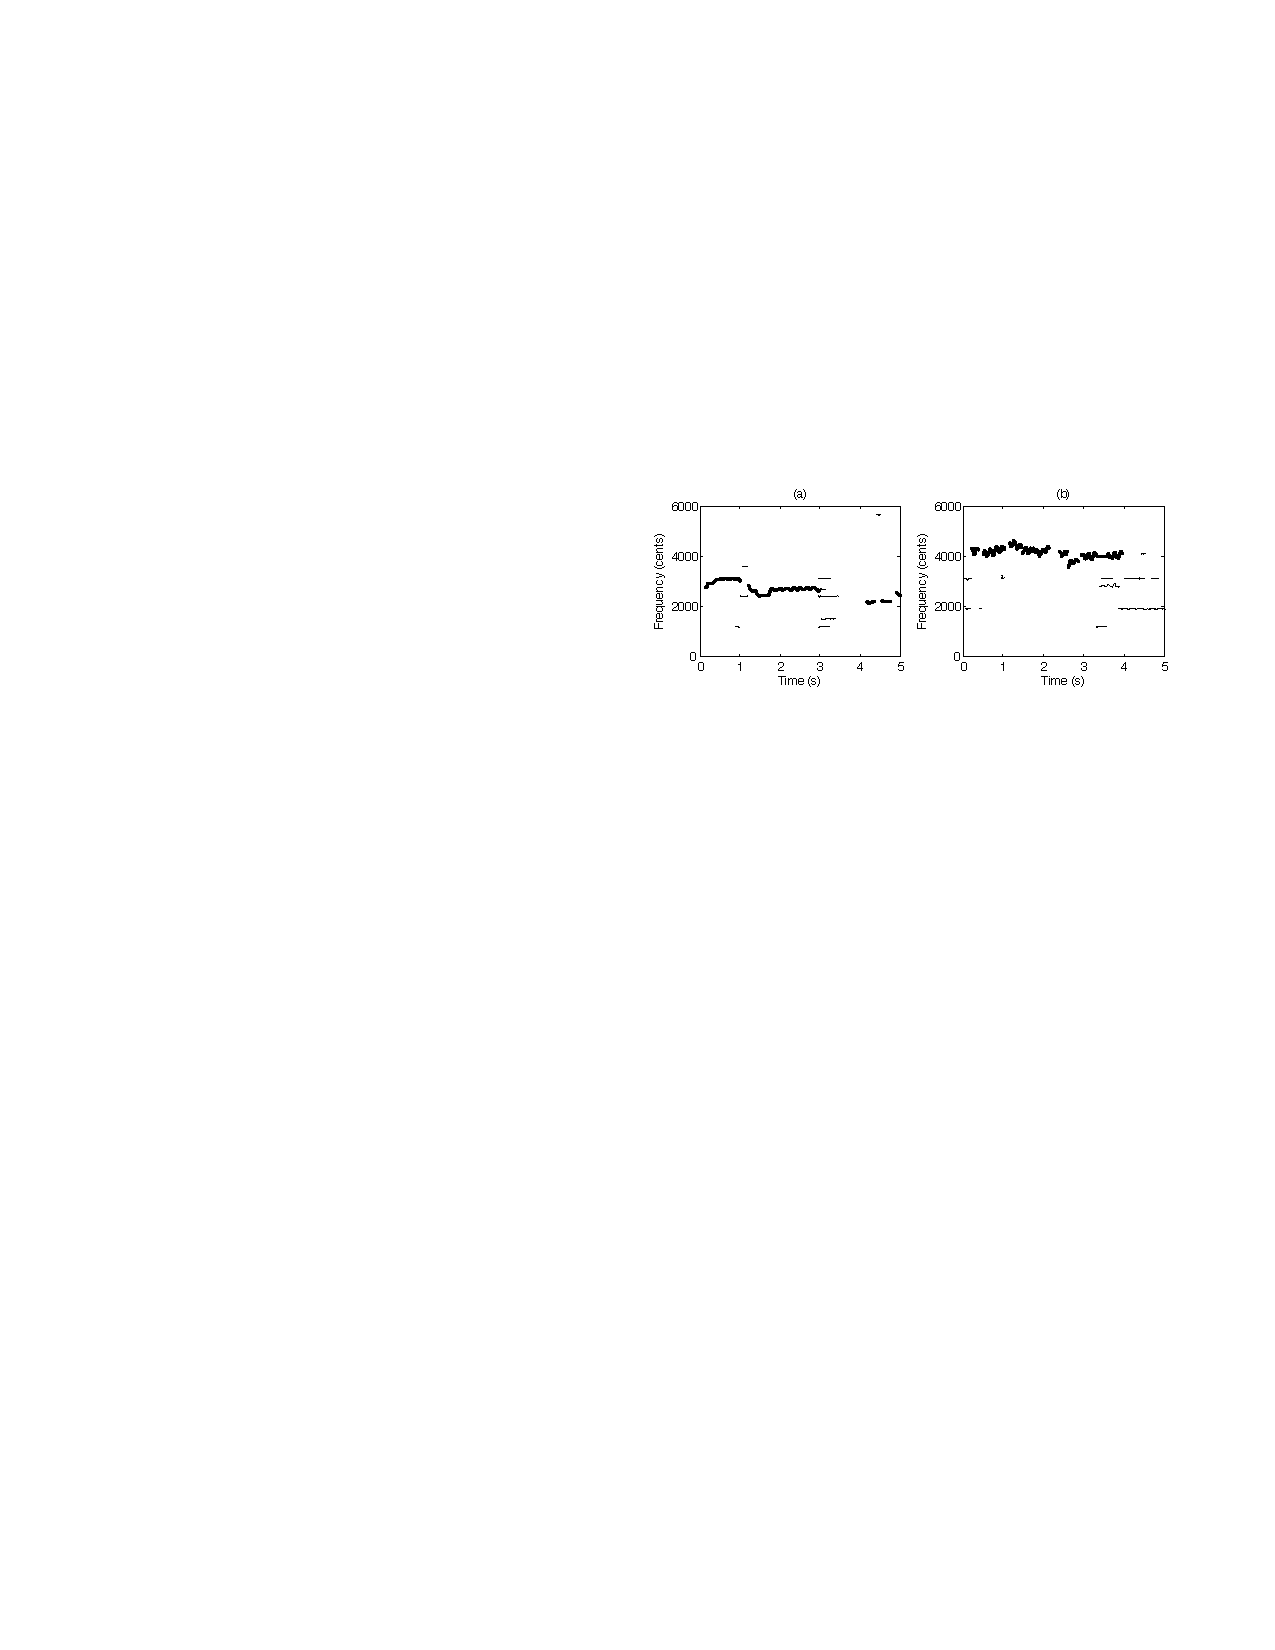
\includegraphics[width=0.7\textwidth]{Figures/pitchcontour}
      \caption{Pitch contours generated from excerpts of (a) vocal jazz and (b) opera. Melody contours are highlighted in bold.}

\end{figure}

To filter out these contours we take advantage of the contour mean salience distribution.
By setting the threshold to a value slightly below the average contour mean salience of all contours in the excerpt $C_{s}$, we can filter out a considerable amount of non-melody contours. We define the following voicing threshold $\tau_{v}$ based on the distribution mean $C_{s}$ and its standard deviation $\sigma_{\overline{s}}$:

$\tau_{v} = C_{s} - v \times \sigma_{\overline{s}}$

The parameter $v$ determines the lenience of the filtering - a high $v$ value might keep the false melody contours and a low value might filter out the melody contours.

It is also important to note that detecting certain characteristics in the contour increases a probability of it being the melody contour, for example in case of detecting a vibrato -  a regular, pulsating change of pitch, used to add expression to vocal and instrumental music. [13]

Next step in the melody selection described by Salamon and G\'{o}mez in their paper is octave errors and pitch outliers removal.  

In particular, the octave errors are the main sources of errors in melody extraction systems, when a multiple or sub-multiple of $f_{0}$ is reported as the main melody. 

To detect such errors, contour trajectories are compared by computing distance between their values on a per-frame for the region they overlap in and computing the mean over this region.
If the mean distance is within $1200\pm50$ cents, the contours are considered octave duplicates.

Secondly, we use the relationship between neighbouring contours (in time) to decide which of the duplicates is the correct one. Our approach is based on two assumptions: firstly, that most (though not all) of the time the correct contour will have greater salience than its duplicate (the salience function parameters were optimised to this end). Secondly, that melodies tend to have a continuous pitch trajectory avoiding large jumps, in accordance with voice leading principles.

The method iteratively computes the $\overline{P(t)}$ - pitch trajectory that represents the time evolution of the melody's pitch.
It then detects and removes an octave duplicate as well as  the "pitch outliers” – contours more than one octave above or below the pitch mean and then it is recalculated. Authors empirically discovered that 2 iterations of this process are enough to get a good approximation of the true trajectory of the melody, which is then passed to the final stage of the model - the final melody selection.

At this stage, there is often only one peak to be chosen as the main melody. When there is still more than one contour present in a frame, the melody is selected as the peak belonging to the contour with the highest total salience $C_{\sum s}$. If no contour is present the frame is regarded as unvoiced.

\begin{figure}[h!]
  \centering
    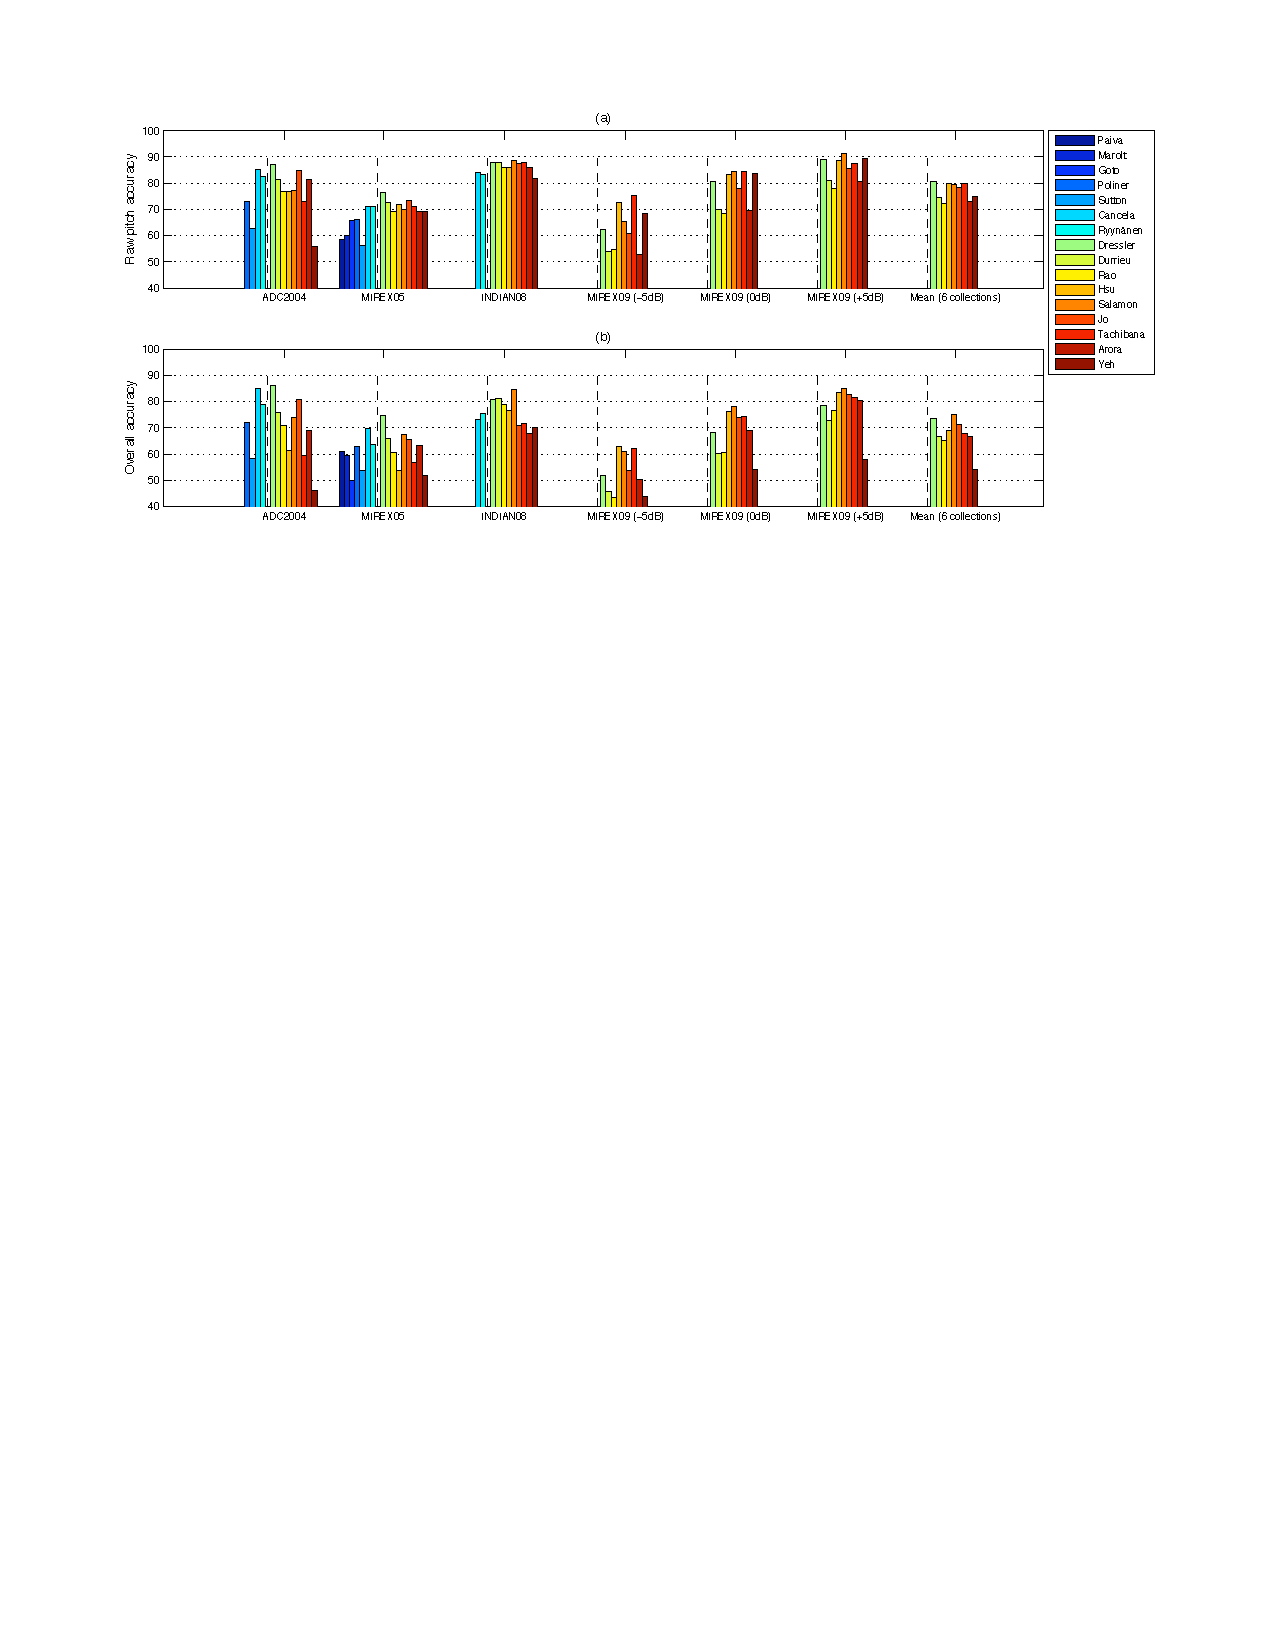
\includegraphics[width=\textwidth]{Figures/comparisonall}
      \caption{a) Raw pitch accuracy and b) overall accuracy obtained in MIREX by 16 melody extraction algorithms evaluated in [14]. Rhe vertical dashed line sepatates the algorithms that were only evaluated on some collections (left of the line) from those evaluated on all six collections (right of the line).}
\end{figure}

\subsection{Comparison of both approaches}

In their paper [14], authors attempted to compare multiple melody extraction algorithms created since 2005. One of the methods, used also by MIREX, is based on the per-frame comparison, considering different measures:

\begin{description}
\item[Voicing Recall Rate] - the proportion of frames labeled as melody frames in the ground truth that are estimated as melody frames by the algorithm.
\item[Voicing False Alarm Rate] - the proportion of the frames labeled as non-melody in the ground truth that are mistakenly estimated as melody frames by the algorithm.
\item[Raw Pitch Accuracy] - the proportion of melody frames in the ground truth for which $f_{\tau}$ is considered correct (i.e. within half a semitone of the ground truth). 
\item[Raw Chroma Accuracy] - as raw pitch accuracy, except that both the estimated and ground truth $f_{0}$ sequences are mapped onto a single octave. This gives a measure of pitch accuracy which ignores octave errors.
\item[Overall Accuracy] - this measure combines the performance of the pitch estimation and voicing detection tasks to give an overall performance score for the system. It is defined as the proportion of all frames correctly estimated by the algorithm, where for non-melody frames this means the algorithm labeled them as non-melody, as for melody frames the algorithm both labeled them as melody frames and provided a correct $f_{0}$ estimate for the melody (again, within half a semitone of the ground truth).
\end{description}

In Figure 2.8. the authors presented results obtained by the algorithms evaluated at MIREX. To get a general idea of the performance of the algorithms it is sufficient to focus on two evaluation measures.
The raw pitch accuracy, presented in Figure 2.8 a) represents how well the algorithm tracks the pitch of the melody. The overall accuracy on the other hand, as shown in Figure 2.8 b), combines this measure with the efficiency of the algorithm's voicing detection, meaning the voicing-related measures are also reflected in this measure.

As we can see, some collections are generally hard to analyse (for example MIREX09 -5db), in general the collections yield different results for different algorithms. This allows us to spot pros and cons of each approach investigated.

We can also notice that the raw pitch accuracy gradually improved from 2005 to 2009, after which it stayed relatively unchanged. Overall we can see that the average pitch accuracy over a collection lies between 70-80%.

On the other hand, when it comes to overall accuracy, the performance goes down compared to the raw pitch accuracy for all algorithms due to voicing detection being factored into the results. The importance of this step depends on the intended use of the algorithm. Generally, the overall accuracy results lie between 65-70%.

Finally, an important factor in assessment of an algorithm is its complexity. While deriving O-notation is too complex for some of the algorithms, generally it is observed that algorithms involving source separation are significantly more computationally complex than salience based approaches, however there is no specific data provided by Salamon and G\'{o}mez [9] or by Durrieu [5] on their algorithms.

In conclusion, we believe the solution proposed by Salamon and G\'{o}mez is better fitted to the purpose of this project. The paper presents it in a much clearer way and, what is most important, it outperforms the one created by Durrieu significantly. In addition to this, according to tendency it is less computationally expensive, which is quite important when it comes to game designing as we do not want to keep the user waiting for a long time for his level to generate and load.

\section{Level Generation}
It is not really surprising that there is no current literature on the problem of automatically generating Guitar Hero buttons given an arbitrary piece of music.
However, we believe an algorithm can be developed where the buttons can be mapped to the $f_{0}$ in the main melody extracted by main melody extraction algorithm.